%Document type: Article
\documentclass[12pt]{article}
\usepackage[utf8]{vietnam}
\usepackage{amsmath}
\usepackage{pdflscape}
\usepackage{lipsum}
\usepackage{epigraph}
\usepackage{amsfonts}
\usepackage{float}
\usepackage{fancyhdr}
\usepackage{graphicx}
\usepackage{setspace}
\usepackage[colorlinks=true,linkcolor=blue, citecolor=red,hypertexnames=false]{hyperref}
\usepackage{url}
\usepackage[top=.75in, left=.75in, right=.75in, bottom=1in]{geometry}
\usepackage{tikz}
\usetikzlibrary{calc}
\usepackage{forest}
\usepackage{multirow}
\usepackage{multicol}
\usepackage{enumerate}
\usepackage{enumitem}
\usepackage{array}
\usepackage[ruled,vlined]{algorithm2e}
%Package for pseudocode 
\usepackage{algpseudocode}

\usepackage{longtable}
\usepackage{booktabs}
\usepackage{xcolor}
\usepackage[most]{tcolorbox}
\usepackage{colortbl}
\usepackage{array}

\usepackage{listings}
\usepackage{proof}
\usetikzlibrary{shapes.geometric, arrows.meta, positioning, calc, shadows}


\definecolor{ui-pink}{RGB}{230, 180, 180}   % Màu hồng cho Label
\definecolor{ui-blue}{RGB}{180, 210, 240}   % Màu xanh cho Value
\definecolor{ui-brown}{RGB}{160, 150, 100}  % Màu nền (nếu cần)
\definecolor{ui-purple}{RGB}{120, 50, 120}  % Màu mũi tên
\definecolor{ui-red}{RGB}{200, 50, 50}      % Màu chữ tiêu đề
\definecolor{accentred}{RGB}{200, 50, 50}
\definecolor{primaryblue}{RGB}{30, 90, 160}
\definecolor{lightgray}{RGB}{245,245,245}
\definecolor{backcolour}{RGB}{245,245,244}
\definecolor{codegreen}{RGB}{0,128,0}
\definecolor{codegray}{RGB}{128,128,128}
\definecolor{codepurple}{RGB}{148,0,211}
\hbadness=10000
\vbadness=10000
\hfuzz=30pt
\vfuzz=400pt
\lstdefinestyle{mystyle}{
    backgroundcolor=\color{backcolour},   
    commentstyle=\color{codegreen},
    keywordstyle=\color{magenta},
    numberstyle=\tiny\color{codegray},
    stringstyle=\color{codepurple},
    basicstyle=\ttfamily\footnotesize,
    breakatwhitespace=false,         
    breaklines=true,                 
    captionpos=b,                    
    keepspaces=true,                 
    numbers=left,                    
    numbersep=5pt,                  
    showspaces=false,                
    showstringspaces=false,
    showtabs=false,                  
    tabsize=2
}

\lstset{style=mystyle}

%Header and Footer
%Set footer
\setlength{\headheight}{29.43912pt}
\pagestyle{fancy}
\fancyfoot{}
\fancyfoot[R]{Page \thepage}

%Left header and right header
\lhead{CANONICAL CORRELATION ANALYSIS}
\rhead{Phân tích thống kê dữ liệu nhiều biến
}

%For Quoting
\makeatletter
\newenvironment{chapquote}[2][2em]
  {\setlength{\@tempdima}{#1}%
   \def\chapquote@author{#2}%
   \parshape 1 \@tempdima \dimexpr\textwidth-2\@tempdima\relax%
   \itshape}
  {\par\normalfont\hfill--\ \chapquote@author\hspace*{\@tempdima}\par\bigskip}
\makeatother

% Key highlighted box with optional title
\newtcolorbox{keybox}[1][]{
  enhanced,
  colback=blue!3,
  colframe=blue!50!black,
  boxrule=0.8pt,
  arc=2pt,
  left=8pt,right=8pt,top=6pt,bottom=6pt,
  title=#1,
  fonttitle=\bfseries
}

%For landscape page
\fancypagestyle{mylandscape}{
\fancyhf{} %Clears the header/footer
\fancyfoot{% Footer
\makebox[\textwidth][r]{% Right
  \rlap{\hspace{.75cm}% Push out of margin by \footskip
    \smash{% Remove vertical height
      \raisebox{4.87in}{% Raise vertically
        \rotatebox{90}{page \thepage}}}}}}% Rotate counter-clockwise
\renewcommand{\headrulewidth}{0pt}% No header rule
\renewcommand{\footrulewidth}{0pt}% No footer rule
}


\usepackage{chngcntr}
\usepackage{titlesec}
% 1. Định dạng lại bộ đếm cho Part thành A, B, C
\renewcommand{\thepart}{\Alph{part}}

% 2. Định dạng lại bộ đếm cho Section thành 1, 2, 3
\renewcommand{\thesection}{\arabic{section}}

% 3. Reset số thứ tự Section mỗi khi sang Part mới
\counterwithin*{section}{part}

% 4. Tùy chỉnh hiển thị (Xóa chữ "Part/Phần", in đậm, màu đỏ)
\titleformat{\part}[block]
  {\bfseries\Large\color{blue}} % Kiểu chữ: Đậm, Lớn, Đỏ
  {\thepart.}                  % Nhãn số: A., B.
  {0.5em}                      % Khoảng cách giữa số và tên
  {}
% Math operators used across chapters
\DeclareMathOperator{\Corr}{Corr}
\DeclareMathOperator{\Cov}{Cov}
\DeclareMathOperator{\Var}{Var}

% Avoid hyperref PDF-string warnings from spacing commands in headings
\pdfstringdefDisableCommands{\def\quad{ }}

%Start the document:
\begin{document}
\begin{titlepage}
\newcommand{\HRule}{\rule{\linewidth}{0.5mm}}
\centering
\textsc{\Large VIETNAM NATIONAL UNIVERSITY HO CHI MINH CITY}\\[0.5cm]
\textsc{\Large UNIVERSITY OF SCIENCE}\\[0.5cm]
\textsc{\large FACULTY OF INFORMATION TECHNOLOGY}\\[0.5cm]

\includegraphics[scale=.30]{Image/hcmus-logo.png}\\[0.5cm] 
\textsc{COMPUTER VISION DEPARTMENT}\\[0.5cm]
\HRule \\[0.4cm]
\huge{\bfseries{CANONICAL CORRELATION ANALYSIS}}\\[0.5cm]
\HRule \\[0.5cm]
\textbf{\large Course: Multivariate Statistical Analysis}\\[0.5cm]
\begin{minipage}[t]{0.4\textwidth}
\begin{flushleft} \large
\emph{Students:}\\
 23127173 - Tran Hai Duc \\
 23127189 - Tran Trong Hieu 
\\ 23127232 - Tran Hoang Nam
\end{flushleft}
\end{minipage}
~
\begin{minipage}[t]{0.4\textwidth}
\begin{flushright} \large
\emph{Supervisor:} \\
Ly Quoc Ngoc
\\ 
\end{flushright}
\end{minipage}\\[1cm]
{\large \today}\\[1cm]
\vfill
\newpage
\end{titlepage}\newpage

\tableofcontents
\pagebreak
\newpage

\part{THEORY}\

\section{Motivation and Context}
\subsection{Overview} Canonical Correlation Analysis (CCA) is a multivariate statistical method to explore and measure the associations between two sets of variables observed on the same group of subjects.
\subsection{Example}
The problem arises from observing two multivariate datasets measured on the same set of subjects (for example, the matrix $\underset{n \times p}{X^{(1)}}$ contains $p=3$ physical exercise indicators (Chins, Situps, Jumps), while the matrix $\underset{n \times q}{X^{(2)}}$ contains $q=2$ physiological indicators (Weight, Waist) for a sample of $n=5$ subjects).
\begin{table}[ht]
    \centering
    \caption{Subset of the Linnerud Dataset ($n=5$)}
    \vspace{0.2cm}
    \begin{tabular}{ccccccc}
        \toprule
        & \multicolumn{3}{c}{Exercise Variables ($X^{(1)}$)} & \multicolumn{2}{c}{Physiological Variables ($X^{(2)}$)} \\
        \cmidrule(lr){2-4} \cmidrule(lr){5-6}
        Subject & Chins ($X^{(1)}_1$) & Situps ($X^{(1)}_2$) & Jumps ($X^{(1)}_3$) & Weight ($X^{(2)}_1$) & Waist ($X^{(2)}_2$) \\
        \midrule
        1 & 5  & 162 & 60  & 191 & 36 \\
        2 & 2  & 110 & 60  & 189 & 37 \\
        3 & 12 & 101 & 101 & 193 & 38 \\
        4 & 12 & 105 & 37  & 162 & 35 \\
        5 & 13 & 155 & 58  & 189 & 35 \\
        \bottomrule
    \end{tabular}
\end{table}

For mathematical computation, the data is structured into two observation matrices, $X^{(1)} \in \mathbb{R}^{5 \times 3}$ and $X^{(2)} \in \mathbb{R}^{5 \times 2}$:

\begin{equation*}
    X^{(1)} = \begin{pmatrix}
    5 & 162 & 60 \\
    2 & 110 & 60 \\
    12 & 101 & 101 \\
    12 & 105 & 37 \\
    13 & 155 & 58
    \end{pmatrix}, \quad
    X^{(2)} = \begin{pmatrix}
    191 & 36 \\
    189 & 37 \\
    193 & 38 \\
    162 & 35 \\
    189 & 35
    \end{pmatrix}
\end{equation*}
% These matrices serve as the foundational inputs to compute the sample covariance matrices ($\Sigma_{11}, \Sigma_{22}, \Sigma_{12}$) required for extracting the canonical weights $\mathbf{a}$ and $\mathbf{b}$.

\subsection{Goals of the CCA}
This study uses CCA with two primary objectives:
\begin{enumerate}[leftmargin=1.8em, label=\textbf{(\arabic*)}]
  \item \textbf{Measure the strength of association between X1 and X2.}
  Rather than relying on isolated pairwise correlations, CCA quantifies the relationship between two multivariate systems through canonical correlation coefficients.

  \item \textbf{Identify informative linear combinations and variable importance.}
  CCA builds linear combinations from X1 and X2 so that their shared variation is maximized. The resulting loading patterns provide interpretable evidence of how strongly each original variable contributes to the cross-set relationship.
\end{enumerate}

\subsection{Research Motivation}

\subsubsection{Scientific Motivation}

\textbf{Continuity with prior research.}
Previous studies have demonstrated that CCA serves as an effective 
denoising mechanism in multi-source data settings, particularly when 
two views describe the same underlying phenomenon under differing 
noise conditions. These findings provide a direct methodological 
foundation for the present work and motivate a principled extension 
of CCA to environmental data.

\textbf{Methodological contributions of CCA.}
From a statistical learning perspective, CCA offers three 
theoretically grounded advantages over conventional single-set 
methods:
\begin{itemize}
    \item \textit{Shared-information-oriented dimensionality 
    reduction}: CCA seeks linear projections that maximize 
    cross-view correlation rather than within-set variance, 
    thereby preserving inter-domain structure that single-set 
    methods would discard.

    \item \textit{Intrinsic noise filtering}: canonical components 
    with low cross-view correlation are suppressed by construction, 
    so view-specific noise is naturally excluded from the learned 
    representation without requiring explicit preprocessing.
\end{itemize}

\subsubsection{Practical Motivation}

\textbf{Applied context: joint analysis of pollutant and 
meteorological data.}
A canonical applied domain for this framework is the joint 
modelling of air-pollutant concentration data and meteorological 
measurements in ground-level ozone research.
Ozone formation is simultaneously governed by emission conditions 
and atmospheric dynamics, constituting a prototypical two-view 
problem in which neither source alone is sufficient for reliable 
analysis.
This structure aligns naturally with the CCA framework, where each 
view captures a distinct but correlated aspect of the same 
environmental process.

\textbf{Practical significance of CCA.}
CCA provides two major practical implications for real-world multi-view analysis:
\begin{itemize}
    \item \textit{Evidence-based variable selection}: by quantifying the strength of association between two variable sets, CCA replaces subjective feature selection with a statistically grounded framework, offering a principled basis for dimensionality reduction and model construction in any multi-view analytical pipeline.

    \item \textit{Improved interpretability and discovery of latent cross-set structure}: by identifying canonical variate pairs with the highest correlation, CCA reveals hidden relationships between two datasets that isolated single-set methods cannot detect. This helps researchers develop a deeper understanding of the data-generating structure and derive conclusions with stronger practical relevance.
\end{itemize}

\subsection{Why CCA Is More Appropriate Than Alternative Approaches}
A common question is why one should not simply concatenate X1 and X2 into a single dataset and compute one overall correlation structure.

The reason is that this pooled strategy mixes two fundamentally different dependency structures:
\begin{itemize}[leftmargin=1.8em]
  \item \textbf{Within-set dependence}: relationships internal to X1 and internal to X2.
  \item \textbf{Between-set dependence}: relationships linking X1 to X2, which is the scientific target.
\end{itemize}

When all variables are merged, strong within-set correlations may dominate and mask the true cross-set signal.
CCA is more appropriate because it directly optimizes the association between X1 and X2 through paired latent directions, while accounting for the variance structure of each set. Therefore, CCA provides a cleaner and more interpretable answer to the central research question: how strongly, and through which latent directions, are X1 and X2 related?

\subsection{Development of CCA problem}

The evolution of CCA can be viewed as a logical progression from simple to complex data structures, moving from analyzing individual points to entire systems:

\begin{enumerate} [leftmargin=1.8em, label=\textbf{(\arabic*)}]
    \item \textbf{1-1 setting (Simple Correlation):} \\
    This is the most fundamental level, focusing on the linear relationship between one variable from $X^{(1)}$ and one variable from $X^{(2)}$. This approach only captures isolated, pairwise connections. Its main limitation is the inability to see the "big picture" when variables within the same set interact with each other, leading to a loss of structural information.

    \item \textbf{1-n setting (Multiple Correlation):} \\
    At this stage, the problem expands to analyze the relationship between the entire set $X^{(1)}$ and only one representative variable from $X^{(2)}$. The goal is to combine all information in $X^{(1)}$ to best explain that single variable. However, this remains asymmetrical; it treats one side as a complex system and the other as a single point, failing to capture the mutual interaction between two multidimensional entities.

    \item \textbf{CCA setting (Multivariate-to-Multivariate):} \\
    This is the most advanced and complete stage, addressing the relationship between the whole set $X^{(1)}$ and the whole set $X^{(2)}$ simultaneously. Instead of picking individual variables, CCA synthesizes all features from both $X^{(1)}$ and $X^{(2)}$ to create "latent variables" that represent each set. The problem evolves into finding the specific "directions" for both sets such that when the data is projected onto them, the correlation between the two systems is maximized. This allows us to quantify the maximum possible "alignment" between two complex data systems, uncovering shared structures that 1-1 or 1-n methods simply cannot detect.
\end{enumerate}





\section{Problem Statement}

The mathematical framework of this study is built upon the principles of Canonical Correlation Analysis (CCA), a sophisticated multivariate statistical technique designed to identify and quantify the underlying associations between two distinct sets of random variables. 

By serving as a strategic extension of Principal Component Analysis (PCA) into a multi-group data context, CCA facilitates the discovery of shared information across different data spaces.


\subsection{ Methodological Foundation and Comparison with PCA}

Principal Component Analysis (PCA) has long been the standard method in multivariate statistics for simplifying large datasets. The core objective of PCA is to address internal variance within a \textbf{single set of variables}. It achieves this by seeking specific directions, known as principal components, such that the variance of the data when projected onto these directions is maximized. In essence, PCA focuses on preserving the maximum amount of information and internal structural variation of an independent data entity, allowing for dimensionality reduction with minimal loss of original features.

However, in many practical scenarios, data does not exist in isolation but appears as pairs of variable sets observed on the same group of subjects. This is where PCA reveals its limitations, as it is not designed to consider the relationship between two different information sources. If we were to apply PCA separately to each set, we might find the most important components for each side, but those components would not necessarily share any meaningful correlation or link with each other.



Canonical Correlation Analysis (CCA) emerged as a strategic extension to address this gap. Unlike PCA, which processes a single set of variables, the primary goal of CCA is to optimize and simplify the relationship between two matrices: 
\begin{equation*}
    X^{(1)} \in \mathbb{R}^{n \times p} \quad \text{and} \quad X^{(2)} \in \mathbb{R}^{n \times q}
\end{equation*}
Instead of searching for directions of maximum variance within each set, CCA focuses on maximizing the correlation between the two. Its objective is to identify pairs of projection directions such that the projection of the first set and the projection of the second set achieve the highest possible degree of alignment or correlation.

The fundamental distinction lies in the optimization philosophy:
\begin{itemize}
    \item \textbf{PCA} is an \textit{inward-looking} problem aimed at finding the best representation of a single system.
    \item \textbf{CCA} is an \textit{outward-looking} problem aimed at finding the strongest connection between two systems.
\end{itemize}

Through this mechanism, CCA is capable of filtering out noise that exists only within individual sets and isolating the strongest common features. This makes CCA a superior tool for uncovering hidden patterns and interactive structures that single-set analysis methods like PCA simply cannot detect.


\subsection{ Input}

The problem formulation of Canonical Correlation Analysis (CCA) begins with two distinct sets of numerical data collected from the same group of $n$ observations. These datasets are represented as two primary data matrices:

\begin{itemize}
    \item \textbf{For the first group ($p$ variables):} The matrix $X^{(1)}$ of dimension $n \times p$ contains $n$ observations across $p$ features.
    \begin{equation}
    X_{n\times p}^{(1)} = \left( X_1^{(1)}, X_2^{(1)}, \dots, X_p^{(1)} \right) = 
    \begin{pmatrix} 
    x_{11}^{(1)} & \dots & x_{1p}^{(1)} \\ 
    \vdots & \ddots & \vdots \\ 
    x_{n1}^{(1)} & \dots & x_{np}^{(1)} 
    \end{pmatrix}
    \end{equation}

    \item \textbf{For the second group ($q$ variables):} The matrix $X^{(2)}$ of dimension $n \times q$ contains the same $n$ observations but measured across $q$ different features.
    \begin{equation}
    X_{n\times q}^{(2)} = \left( X_1^{(2)}, X_2^{(2)}, \dots, X_q^{(2)} \right) = 
    \begin{pmatrix} 
    x_{11}^{(2)} & \dots & x_{1q}^{(2)} \\ 
    \vdots & \ddots & \vdots \\ 
    x_{n1}^{(2)} & \dots & x_{nq}^{(2)} 
    \end{pmatrix}
    \end{equation}
\end{itemize}

\paragraph{The Joint Covariance Structure}


To analyze the relationship between these two matrices, the fundamental input used in the mathematical computation is the partitioned joint covariance matrix $\Sigma$. This matrix captures both the internal variance of each set and the cross-set interactions:
\begin{equation}
\Sigma = \begin{pmatrix} 
\Sigma_{11} & \Sigma_{12} \\ 
\Sigma_{21} & \Sigma_{22} 
\end{pmatrix}
\end{equation}
Where:
\begin{itemize}
    \item $\Sigma_{11}$ ($p \times p$) and $\Sigma_{22}$ ($q \times q$) represent the within-set covariance matrices for $X^{(1)}$ and $X^{(2)}$, respectively.
    \item $\Sigma_{12}$ ($p \times q$) and its transpose $\Sigma_{21}$ ($q \times p$) represent the cross-set covariance matrices, which encapsulate the linear dependencies between the two groups.
\end{itemize}

\paragraph{Construction of Canonical Variates}
From these primary inputs, CCA seeks to synthesize the high-dimensional data into a more manageable and interpretable form. We construct aggregate variables, known as canonical variable vectors $U$ and $V$, through the following linear combinations:
\begin{equation}
U_{n\times 1} = X_{n\times p}^{(1)} a_{p\times 1} \quad \text{and} \quad V_{n\times 1} = X_{n\times q}^{(2)} b_{q\times 1}
\end{equation}
In this transformation:
\begin{itemize}
    \item $a$ and $b$ are the weight vectors that determine the direction of the projection in each respective variable space.
    \item $U$ and $V$ are the resulting column vectors representing the scores of the $n$ observations on these new canonical dimensions.
\end{itemize}

The input stage effectively sets the foundation for the optimization process: we use the raw data matrices to derive the covariance structure, which then allows us to find the optimal weights $a$ and $b$ that align $U$ and $V$ as closely as possible.


\subsection{Output}

The objective of Canonical Correlation Analysis is to determine two sets of coefficient vectors, known as the canonical weight vectors,

\begin{equation*}
\mathbf{a} \in \mathbb{R}^{p \times 1}, \qquad 
\mathbf{b} \in \mathbb{R}^{q \times 1},
\end{equation*}

which define the canonical variables

\begin{equation*}
U = X^{(1)}\mathbf{a}, \qquad 
V = X^{(2)}\mathbf{b}.
\end{equation*}

These linear combinations represent aggregated variables that summarize each dataset while emphasizing their shared variation.


\paragraph{The Correlation Metric}
The strength of association between the two canonical variables is measured by the canonical correlation $\rho$:
\begin{equation}
\rho = \text{Corr}(U,V) = \frac{\text{Cov}(U,V)}{\sqrt{\text{Var}(U)\text{Var}(V)}} = \frac{\mathbf{a}^T \Sigma_{12} \mathbf{b}}{\sqrt{\mathbf{a}^T \Sigma_{11} \mathbf{a}} \sqrt{\mathbf{b}^T \Sigma_{22} \mathbf{b}}}
\end{equation}

Equation defines the correlation metric between two multivariate spaces through the following components:
\begin{itemize}
    \item \textbf{The Covariance Term ($\text{Cov}(U,V)$):} The numerator measures the shared information between the two datasets. It represents the degree to which the canonical variate $U$ (derived from the first group) and $V$ (derived from the second group) co-vary, capturing the linear dependency extracted via the cross-covariance structure.

    \item \textbf{The Normalization Factor ($\sqrt{\text{Var}(U)\text{Var}(V)}$):} The denominator serves as a scaling mechanism using the product of the standard deviations of the constructed variables. This ensures that the canonical correlation $\rho$ is constrained within the interval $[0, 1]$, allowing for an objective assessment of the association that is invariant to the original units or scales of the input variables.
\end{itemize}

The CCA problem is therefore to determine the vectors $\mathbf{a}$ and $\mathbf{b}$ such that correlation of $U$ and $V$ is as large as possible:

\begin{equation}
\rho = 
\max_{\mathbf{a},\mathbf{b}}
\text{Corr}(X^{(1)}\mathbf{a}, X^{(2)}\mathbf{b}).
\end{equation}

This optimization serves as the core objective of the framework. Instead of calculating correlations between every individual pair of variables, CCA identifies the optimal directions within the multidimensional space of each dataset such that their projections onto these directions are as similar as possible. Through this process, CCA transforms the complex interaction between the two variable groups into a single interpretable measure of association.
\paragraph{Multiple Canonical Pairs}


In general, Canonical Correlation Analysis does not produce a single pair of canonical variables. 
Given two variable sets of dimensions $p$ and $q$, the method can generate at most

\begin{equation}
k = \min(p, q)
\end{equation}

Where: p = Rank(X) and q = Rank(Y).

pairs of canonical variables:

\begin{equation}
(U_1,V_1), (U_2,V_2), \dots, (U_k,V_k).
\end{equation}

The number of canonical pairs $k$ is constrained by the minimum value of $p$ and $q$ due to fundamental algebraic and geometric limitations. Specifically, the statistical interaction is captured by the $p \times q$ cross-covariance matrix $\Sigma_{12}$. Since the rank of this matrix cannot exceed its smallest dimension, the number of independent informational components is limited to $\min(p, q)$. Furthermore, each subsequent pair $(U_i, V_i)$ must remain uncorrelated with all previous pairs. Once the degrees of freedom in the smaller dataset are exhausted, no further orthogonal directions can be identified to form additional pairs.

Each pair is associated with a canonical correlation coefficient

\begin{equation}
\rho_1 \ge \rho_2 \ge \dots \ge \rho_k,
\end{equation}

where the first pair $(U_1,V_1)$ maximizes the correlation between the two datasets, and subsequent pairs are obtained under the additional constraint of being uncorrelated with the previous canonical variables.



\subsection{Constraints and the Strategic Role of Normalization}

To ensure a unique and stable solution while maintaining comparability across different scales of measurement, Canonical Correlation Analysis imposes a set of fundamental constraints on the construction of the canonical variates.

\paragraph{Unit-Variance Constraints}
The primary constraint is to normalize the canonical variates $U$ and $V$ to have unit variance. This eliminates the arbitrary scaling effects of the original variables:
\begin{equation}
\text{Var}(U) = \mathbf{a}^T \Sigma_{11} \mathbf{a} = 1
\end{equation}
\begin{equation}
\text{Var}(V) = \mathbf{b}^T \Sigma_{22} \mathbf{b} = 1
\end{equation}
where $\Sigma_{11}$ and $\Sigma_{22}$ represent the within-set covariance matrices. These constraints prevent variables with large numerical ranges from disproportionately influencing the results, shifting the analytical focus toward intrinsic interactions.

\paragraph{Orthogonality and Uncorrelatedness}
When extracting multiple pairs of canonical variables $(U_k, V_k)$, additional constraints are required to ensure that each pair captures unique information. To achieve a non-redundant decomposition of the relationship between the two datasets, each new pair must be uncorrelated with all previously identified pairs:

\begin{align}
    \text{Cov}(U_k, U_l) &= 0, \quad \forall k \neq l; \quad k, l = 1, 2, \dots, p \\
    \text{Cov}(V_k, V_l) &= 0, \quad \forall k \neq l; \quad k, l = 1, 2, \dots, q \\
    \text{Cov}(U_k, V_l) &= 0, \quad \forall k \neq l; \quad k, l = 1, 2, \dots, \min(p, q)
\end{align}



These constraints establish a framework where the canonical variates within the same group remain linearly independent to represent distinct directions of variance. Furthermore, they ensure that a canonical variate from one group exhibits zero correlation with any variate from the other group, except for its specific partner. This structured approach isolates each mode of interaction into independent channels, which are then ordered by their strength of correlation $\rho_k$.



\paragraph{Strategic Role of Normalization}
Mathematically, when variances are normalized to unity, the correlation coefficient converges directly to the covariance:
\begin{equation}
\text{Corr}(U, V) \rightarrow \text{Cov}(U, V)
\end{equation}
This provides a pure reflection of the structural similarity between the two groups. By enforcing these constraints, CCA transforms the optimization problem into a well-posed generalized eigenvalue problem, ensuring that the resulting canonical correlations $\rho_i$ are invariant to linear scaling of the original data.


\section{Method}
Canonical correlation analysis originates in Hotelling (1936) and the two equations that govern the analysis are the following:
\begin{equation} \label{eq:cca_final_b}
    (\Sigma_{21} \Sigma_{11}^{-1} \Sigma_{12} - \rho^2 \Sigma_{22})\mathbf{b} = 0
\end{equation}
\begin{equation} \label{eq:cca_final_a}
    (\Sigma_{12} \Sigma_{22}^{-1} \Sigma_{21} - \rho^2 \Sigma_{11})\mathbf{a} = 0
\end{equation}
where $\Sigma_{21} = \Sigma_{12}^T$. Both equations look similar and have, in fact, the same eigenvalues. And, given the eigenvectors for one of these equations, we can deduce the eigenvectors for the other as will be shown in the next section.

\subsection{Derivation of the canonical correlation analysis equations}
In canonical correlation analysis, we want to maximize correlations between objects that are represented with two data sets. Let us consider two groups of random variables:
\begin{itemize}
    \item Group 1: $\underset{1 \times p}{\mathbf{X}}^{(1)} = (X_1^{(1)}, X_2^{(1)}, \dots, X_p^{(1)})$
    \item Group 2: $\underset{1 \times q}{\mathbf{X}}^{(2)} = (X_1^{(2)}, X_2^{(2)}, \dots, X_q^{(2)})$
\end{itemize}
Sometimes the data in $\mathbf{X}^{(2)}$ and $\mathbf{X}^{(1)}$ are called the dependent and the independent data, respectively. The maximum number of correlations that we can find is then equal to the minimum of the dimensions $p$ and $q$.

Let the directions of optimal correlations for the $\mathbf{X}^{(1)}$ and $\mathbf{X}^{(2)}$ data sets be given by the coefficient vectors $\mathbf{a}$ and $\mathbf{b}$, respectively. We consider the linear combinations $U$ and $V$, defined as follows:
\begin{equation} \label{eq:U_def}
    \underset{1 \times 1}U =  \underset{1 \times p}{\mathbf{X}}^{(1)}\underset{p \times 1} {\mathbf{a}}
\end{equation}
\begin{equation} \label{eq:V_def}
    \underset{1 \times 1}V =  \underset{1 \times q}{\mathbf{X}}^{(2)}\underset{q \times 1} {\mathbf{b}}
\end{equation}

The variables $U$ and $V$ are called the canonical variates. The correlation between them is defined as

\begin{equation}
\rho = \frac{\text{Cov}(U,V)}{\sqrt{\text{Var}(U)\text{Var}(V)}} .
\end{equation}

Since $U = X^{(1)}a$ and $V = X^{(2)}b$, we can express the covariance as

\begin{equation}
\text{Cov}(U,V) 
= \text{Cov}( \mathbf{X}^{(1)} \mathbf{a},  \mathbf{X}^{(2)} \mathbf{b}) 
= \underset{1 \times p}{\mathbf{a}^T} \, \underset{p \times q}{\text{Cov}(\mathbf{X}^{(1)}, \mathbf{X}^{(2)})} \, \underset{q \times 1}{\mathbf{b}}
= \underset{1 \times p}{\mathbf{a}^T} \, \underset{p \times q}{\Sigma_{12}} \, \underset{q \times 1}{\mathbf{b}}
\end{equation}
Similarly, the variances of $U$ and $V$ are

\begin{equation}
\text{Var}(U) = \text{Var}(X^{(1)}a)
= a^T \Sigma_{11} a
\end{equation}

\begin{equation}
\text{Var}(V) = \text{Var}(X^{(2)}b)
= b^T \Sigma_{22} b .
\end{equation}

Substituting these expressions into the definition of correlation yields

\begin{equation} \label{eq:rho_formula}
\rho =
\frac{a^T \Sigma_{12} b}
{\sqrt{a^T \Sigma_{11} a \; b^T \Sigma_{22} b}} .
\end{equation}
Our problem is now finding the directions $\mathbf{b}$ and $\mathbf{a}$ that maximize equation \eqref{eq:rho_formula} above.

We first note that $\rho$ is not affected by a rescaling of $V$ or $U$. Since the choice of rescaling is arbitrary, we therefore maximize equation \eqref{eq:rho_formula} subject to the constraints:
\begin{equation} \label{eq:const_u}
    \text{Var}(U) = \underset{1 \times p}{\mathbf{a}^T} \underset{p \times p}{\Sigma_{11}} \underset{p \times 1}{\mathbf{a}} = 1
\end{equation}
\begin{equation} \label{eq:const_v}
    \text{Var}(V) = \underset{1 \times q}{\mathbf{b}^T} \underset{q \times q}{\Sigma_{22}} \underset{q \times 1}{\mathbf{b}} = 1
\end{equation}
We have made the substitutions where the $\Sigma$'s are covariance matrices. We write the maximization problem in Lagrangian form:
\begin{equation} \label{eq:lagrangian}
    L(\rho_a, \rho_b, \mathbf{a}, \mathbf{b}) = \mathbf{b}^T \Sigma_{21} \mathbf{a} - \frac{\rho_a}{2}(\mathbf{a}^T \Sigma_{11} \mathbf{a} - 1) - \frac{\rho_b}{2}(\mathbf{b}^T \Sigma_{22} \mathbf{b} - 1)
\end{equation}
To solve equation \eqref{eq:lagrangian}, we take partial derivatives with respect to $\mathbf{a}$ and $\mathbf{b}$ and set them to zero:

\begin{equation} \label{eq:deriv_a}
    \frac{\partial L}{\partial \mathbf{a}} = (\mathbf{b}^T\Sigma_{21})^T - \frac{\rho_a}{2} (2 \Sigma_{11} \mathbf{a}) = \Sigma_{12} \mathbf{b} - \rho_a \Sigma_{11} \mathbf{a} = 0 \implies \underset{p \times q}{\Sigma_{12}} \underset{q \times 1}{\mathbf{b}} = \rho_a \underset{p \times p}{\Sigma_{11}} \underset{p \times 1}{\mathbf{a}}
\end{equation}
\begin{equation} \label{eq:deriv_b}
    \frac{\partial L}{\partial \mathbf{b}} = \Sigma_{12}^T \mathbf{a} - \frac{\rho_b}{2} (2 \Sigma_{22} \mathbf{b}) = \Sigma_{21} \mathbf{a} - \rho_b \Sigma_{22} \mathbf{b} = 0 \implies \underset{q \times p}{\Sigma_{21}} \underset{p \times 1}{\mathbf{a}} - \rho_b \underset{q \times q}{\Sigma_{22}} \underset{q \times 1}{\mathbf{b}}
\end{equation}




To identify the relationship between the multipliers $\rho_a$ and $\rho_b$, we left-multiply \eqref{eq:deriv_a} by $\mathbf{a}^T$ and \eqref{eq:deriv_b} by $\mathbf{b}^T$:
\begin{itemize}
    \item From \eqref{eq:deriv_a}: $\mathbf{a}^T \Sigma_{12} \mathbf{b} = \rho_a (\mathbf{a}^T \Sigma_{11} \mathbf{a})$. Given the constraint \eqref{eq:const_u}, we have $\rho_a = \mathbf{a}^T \Sigma_{12} \mathbf{b}$.
    \item From \eqref{eq:deriv_b}: $\mathbf{b}^T \Sigma_{21} \mathbf{a} = \rho_b (\mathbf{b}^T \Sigma_{22} \mathbf{b})$. Given the constraint \eqref{eq:const_v}, we have $\rho_b = \mathbf{b}^T \Sigma_{21} \mathbf{a}$.
\end{itemize}
Since $\mathbf{a}^T \Sigma_{12} \mathbf{b}$ is a scalar, it is equal to its transpose: $(\mathbf{a}^T \Sigma_{12} \mathbf{b})^T = \mathbf{b}^T \Sigma_{12}^T \mathbf{a} = \mathbf{b}^T \Sigma_{21} \mathbf{a}$. This implies that:
\begin{equation} \label{eq:rho_equality}
    \rho_a = \rho_b = \rho = \text{Cov}(U, V)
\end{equation}
Thus, the Lagrange multipliers are identical and equal to the canonical correlation we seek to maximize. Assuming $\Sigma_{11}$ is non-singular, we can rearrange \eqref{eq:deriv_a} to express $\mathbf{a}$ in terms of $\mathbf{b}$:
\begin{equation} \label{eq:a_sol}
\Sigma_{12} \mathbf{b} = \rho_a \Sigma_{11} \mathbf{a} \implies \mathbf{a} = \frac{\Sigma_{11}^{-1} \Sigma_{12} \mathbf{b}}{\rho}
\end{equation}
Substituting \eqref{eq:a_sol} into \eqref{eq:deriv_b} yields the generalized eigenvalue problem for $\mathbf{b}$:
\begin{equation} \label{eq:gen_eig_b}
     \Sigma_{21} \mathbf{a} = \rho_b \Sigma_{22} \mathbf{b} \implies \Sigma_{21} \left( \frac{\Sigma_{11}^{-1} \Sigma_{12} \mathbf{b}}{\rho} \right) = \rho \Sigma_{22} \mathbf{b} \implies (\Sigma_{21} \Sigma_{11}^{-1} \Sigma_{12} - \rho^2 \Sigma_{22})\mathbf{b} = 0
\end{equation}

In an analogous way, we can get the equation for the vectors $\mathbf{a}$ as:
\begin{equation} \label{eq:gen_eig_a}
    (\Sigma_{12} \Sigma_{22}^{-1} \Sigma_{21} - \rho^2 \Sigma_{11})\mathbf{a} = 0
\end{equation}
These equations are so called generalized eigenvalue problems. Special software is needed to solve these equations in a numerically stable and robust manner.

\subsection{Solution of the population CCA problem}
Equation \eqref{eq:gen_eig_b} has the form of a generalized eigenvalue problem
\[
A\mathbf{b} = \lambda B\mathbf{b},
\]
where
\[
A = \Sigma_{21}\Sigma_{11}^{-1}\Sigma_{12}, \quad
B = \Sigma_{22}, \quad
\lambda = \rho^2.
\]
We can consider two cases here: the simple case when we only have the covariance matrices, or, the somewhat more involved case, when we have the original data matrices at our disposal.
If $\Sigma_{22}$ is non-singular, the generalized eigenvalue problem
can be converted into a standard eigenvalue problem by multiplying
\eqref{eq:gen_eig_b} from the left by $\Sigma_{22}^{-1}$, yielding

\begin{equation} \label{eq:eig_standard_b}
    (\Sigma_{22}^{-1} \Sigma_{21} \Sigma_{11}^{-1} \Sigma_{12} - \rho^2 I)\mathbf{b} = 0
\end{equation}

Equation \eqref{eq:eig_standard_b} is a standard eigenvalue problem of the form

\[
M \mathbf{b} = \rho^2 \mathbf{b},
\]

where

\[
M = \Sigma_{22}^{-1} \Sigma_{21} \Sigma_{11}^{-1} \Sigma_{12}.
\]

Thus, the canonical correlations can be obtained by solving the
eigenvalue problem for the matrix $M$. Let

\[
M \mathbf{b}_i = \lambda_i \mathbf{b}_i ,
\]

where $\lambda_i$ are the eigenvalues and $\mathbf{b}_i$ the corresponding
eigenvectors. The canonical correlations are then given by

\[
\rho_i = \sqrt{\lambda_i}.
\]

Once the vectors $\mathbf{b}_i$ are obtained, the corresponding vectors
$\mathbf{a}_i$ can be computed from equation \eqref{eq:deriv_a} as

\[
\mathbf{a}_i =
\frac{\Sigma_{11}^{-1} \Sigma_{12} \mathbf{b}_i}{\rho_i}.
\]

The vectors $\mathbf{a}_i$ and $\mathbf{b}_i$ define the canonical
directions, and the corresponding canonical variates are

\[
U_i = \mathbf{a}_i^T \mathbf{X}^{(1)}, \qquad
V_i = \mathbf{b}_i^T \mathbf{X}^{(2)} .
\]

The number of non–zero canonical correlations is at most
$\min(p,q)$.


\subsection{Solution of the sample CCA problem }
In practical applications, the true population parameters are unknown. We estimate the canonical correlations and weights using the full Linnerud dataset n=20.
\subsubsection{Data Centering}
 Let $\mathbf{X}^{(1)} \in \mathbb{R}^{n \times p}$ and $\mathbf{X}^{(2)} \in \mathbb{R}^{n \times q}$ be the observed data matrices. For CCA to correctly identify relationships based on variance, the data must first be centered:
\begin{equation}
\bar{\mathbf{X}}^{(1)} =
\mathbf{X}^{(1)} -
\begin{pmatrix}
1\\
1\\
\vdots\\
1
\end{pmatrix}
\boldsymbol{\mu}^{(1)},
\quad
\bar{\mathbf{X}}^{(2)} =
\mathbf{X}^{(2)} -
\begin{pmatrix}
1\\
1\\
\vdots\\
1
\end{pmatrix}
\boldsymbol{\mu}^{(2)}
\end{equation}
 where $\boldsymbol{\mu}$ represents the vector of column means. This ensures that the variables have a mean of zero, allowing the subsequent matrix products to represent covariances.
 \subsubsection{Sample Covariance Estimation}
 The sample covariance matrices are estimated from the centered data as follows:\begin{equation}\hat{\Sigma}_{11} = \frac{1}{n-1}\bar{\mathbf{X}}^{(1)T}\bar{\mathbf{X}}^{(1)}, \quad \hat{\Sigma}_{22} = \frac{1}{n-1}\bar{\mathbf{X}}^{(2)T}\bar{\mathbf{X}}^{(2)}, \quad \hat{\Sigma}_{12} = \frac{1}{n-1}\bar{\mathbf{X}}^{(1)T}\bar{\mathbf{X}}^{(2)}
\end{equation}
where $\hat{\Sigma}_{11} \in \mathbb{R}^{p \times p}$ and $\hat{\Sigma}_{22} \in \mathbb{R}^{q \times q}$ represent the internal variance structures, and $\hat{\Sigma}_{12} \in \mathbb{R}^{p \times q}$ captures the cross-set associations.\subsubsection{ Solving the Empirical Eigenvalue Problem}
We solve for the sample canonical weights by substituting the estimates into the standard eigenvalue problem:\begin{equation} \label{eq:sample_eig_b}(\hat{\Sigma}_{22}^{-1} \hat{\Sigma}_{21} \hat{\Sigma}_{11}^{-1} \hat{\Sigma}_{12}) \hat{\mathbf{b}}_i = \hat{\rho}_i^2 \hat{\mathbf{b}}i
\end{equation}
The sample canonical correlations $\hat{\rho}_i$ are the square roots of the eigenvalues. The weight vectors $\hat{\mathbf{a}}_i$ for the exercise set are then recovered:
\begin{equation}
\hat{\mathbf{a}}_i = \frac{\hat{\Sigma}_{11}^{-1} \hat{\Sigma}_{12} \hat{\mathbf{b}}_i}{\hat{\rho}_i}\end{equation}
\subsubsection{ Computation of Sample Scores}
The final canonical scores for the 20 subjects are obtained by projecting the centered data onto the estimated canonical directions:\begin{equation}\hat{\mathbf{u}}_i = \bar{\mathbf{X}}^{(1)} \hat{\mathbf{a}}_i, \qquad \hat{\mathbf{v}}_i = \bar{\mathbf{X}}^{(2)} \hat{\mathbf{b}}_i\end{equation}These scores $\hat{\mathbf{u}}_i, \hat{\mathbf{v}}_i \in \mathbb{R}^{n}$ provide a simplified, one-dimensional representation of each subject's position along the identified latent axes of "Physical Effort" and "Physiological Profile".
\subsection{Hypothesis Testing and Statistical Significance}

After calculating the sample canonical correlations $\hat{\rho}_i$, we must determine whether these associations represent true relationships in the population or are merely products of sampling error.
\subsubsection{Overall Test of Independence}
The primary hypothesis tests whether there is any linear relationship between the two sets of variables:\begin{itemize}\item $H_0: \rho_1 = \rho_2 = \dots = \rho_k = 0$ (The two sets are independent)\item $H_1: \text{At least one } \rho_i \neq 0$ (There is at least one significant association)\end{itemize}where $k = \min(p, q)$.
\subsubsection{Wilks' Lambda Statistic}
The test is based on Wilks' Lambda ($\Lambda$), which measures the proportion of variance not explained by the canonical variables. It is calculated using the sample correlations:\begin{equation}\Lambda_1 = \prod_{i=1}^{k} (1 - \hat{\rho}_i^2)\end{equation}A value of $\Lambda$ near $0$ indicates a strong association, while a value near $1$ suggests independence.
\subsubsection{Bartlett's Chi-square Transformation}
For large samples, Bartlett proposed a transformation of $\Lambda$ to a Chi-square distribution to simplify the calculation of $p$-values. The test statistic is given by:\begin{equation}\chi^2 = - \left( n - 1 - \frac{p + q + 1}{2} \right) \ln \Lambda_1\end{equation}This statistic follows a Chi-square distribution with $\mathbf{df = p \times q}$ degrees of freedom.
\subsubsection{Sequential Testing (Dimension Reduction)}
If the overall $H_0$ is rejected, we conclude that the first pair of canonical variables is significant. We then proceed to test if the remaining correlations are significant by "peeling off" the first one:\begin{equation}\Lambda_m = \prod_{i=m}^{k} (1 - \hat{\rho}_i^2)\end{equation}The degrees of freedom for each subsequent step $m$ are adjusted to:\begin{equation}df = (p - m + 1)(q - m + 1)\end{equation}This sequential process allows us to determine the exact number of significant canonical dimensions to interpret.
\subsubsection{Application to Linnerud Dataset }
For the full Linnerud dataset ($p=3, q=2$), we have:\begin{itemize}\item Step 1: Overall test ($m=1$) with $df = 3 \times 2 = 6$.\item Step 2: Testing the remaining correlation ($m=2$) with $df = (3-1)(2-1) = 2$.\end{itemize}If the $p$-value for Step 1 is less than the significance level (e.g., $\alpha = 0.05$), we reject the null hypothesis and proceed to interpret the first canonical dimension.
\section{Geometric Meaning}

The figure below provides a geometric interpretation of Canonical Correlation Analysis (CCA). 
In this illustration, $x_1, x_2$ are the original variables (columns) belonging to dataset $X$, 
and $y_1, y_2$ are the original variables (columns) belonging to dataset $Y$. 
Each dataset is represented as a subspace — here depicted as a two-dimensional plane, 
since each dataset contains two columns. The vectors $\mathbf{V}_X$ and $\mathbf{V}_Y$ 
correspond to the canonical variates $U$ and $V$, respectively — the linear combinations 
of the original variables that CCA seeks to find.

\begin{figure}[ht]
    \centering
    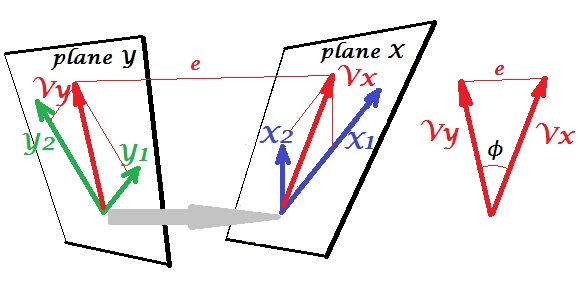
\includegraphics[width=0.7\textwidth]{Image/geometry.jpg}
    \caption{Geometric interpretation of CCA. The datasets $X$ and $Y$ span two separate 
    subspaces (planes). The canonical variates $\mathbf{V}_X$ and $\mathbf{V}_Y$ are the 
    directions within each plane that minimize the angle $\phi$ between them.}
    \label{fig:geometric_cca}
\end{figure}

The key geometric insight of CCA is as follows. Rather than analyzing each dataset in 
isolation, CCA looks for the relationship \emph{between} the two subspaces. Specifically, 
it identifies the pair of directions — one in the subspace of $X$ and one in the subspace 
of $Y$ — such that the angle $\phi$ between them is minimized. The canonical correlation 
$\rho$ is then defined as the cosine of this angle:
\[
    \rho = \cos(\phi).
\]

Two subspaces are said to be \emph{maximally correlated} when they are parallel, i.e., 
when the angle between them equals zero ($\phi = 0$, so $\rho = 1$). In this case, the 
two linear combinations $U = \mathbf{V}_X^\top X$ and $V = \mathbf{V}_Y^\top Y$ point 
in the same direction, indicating a perfect linear relationship between the two datasets. 
Conversely, when the subspaces are orthogonal ($\phi = 90^\circ$, $\rho = 0$), the datasets 
are uncorrelated.

The line $e$ in the figure represents the residual — the component that remains after 
projecting one canonical variate onto the other. Minimizing $e$ is equivalent to 
maximizing the canonical correlation $\rho$, which is precisely the objective of CCA.

In summary, CCA can be interpreted geometrically as finding the \emph{closest pair of 
directions} between two subspaces, where closeness is measured by the angle between them.
\section{Kiểm chứng tính đúng đắn}
\input{chapter_part_A/Ví dụ}
\newpage
\part{EXPERIMENTAL APPLICATIONS}
\section{Problem Statement}

\subsection{Introduction}
In the context of the increasing prevalence of speech recognition technology, processing audio signals in real-world environments remains a significant challenge due to the impact of unwanted noise. This research focuses on applying Canonical Correlation Analysis as a powerful preprocessing technique to enhance the input quality for Speech-to-Text systems. Unlike traditional noise filtering methods that often focus on frequency suppression, CCA aims to identify and establish links between multi-dimensional data sources. This allows the system to recognize and preserve the core invariant features of human speech, even when they are obscured by complex noise components.

The primary objective of this experiment is to use CCA to learn these invariant features, which are the most stable and essential signal components of speech. By maximizing the correlation between reference datasets, the study aims to build an intelligent filter capable of automatically separating the target signal from random environmental noise without requiring strict assumptions about the type of noise involved. The final result is a preprocessing solution that significantly improves the accuracy of the output text, ensuring the robustness of the recognition system even when the input audio quality is severely degraded by external factors.

\subsection{Input}
The experimental procedure was designed in two distinct phases to optimize recognition capabilities.

\subsubsection{Training Phase}
The experimental workflow begins with a training phase designed to build an optimal signal separation model using paired reference data. During this stage, the system simultaneously processes two input datasets:
\begin{itemize}
    \item \textbf{Clean Dataset ($X^{(1)}$):} Consists of standard audio samples recorded in an ideal, noise-free environment.
    \item \textbf{Noisy Dataset ($X^{(2)}$):} Generated by integrating Additive White Gaussian Noise (AWGN) directly into the clean samples.
\end{itemize}

Simulating noise in this manner allows for precise control over data variability, creating a complete experimental environment for the algorithm to learn the mapping between the clean entity and its noisy counterpart. The core role of using the clean and noisy data pair is to provide the CCA method with a precise frame of reference to define the stable mathematical structure of human speech. Through the mechanism of maximizing covariance, CCA learns to focus on the components with the highest correlation between the two datasets (the target signal) while automatically identifying and suppressing uncorrelated random fluctuations (the noise components). The outcome of this phase is an optimized set of canonical weights, acting as a feature map that enables the system to retrieve useful information from chaotic data sources in subsequent execution stages.

\subsubsection{Testing Phase}
Once the optimal canonical weights have been established during the training phase, the system is deployed for real-world recognition tasks using individual audio sources. In this phase, the input data can be any environmental audio signal, which is often degraded by ambient noise or white noise. 

Instead of attempting to reconstruct a clean acoustic waveform, the system applies the learned projection matrices to transform the noisy audio data into a new feature space. Within this space, CCA functions by filtering out irrelevant noise fluctuations and preserving only the signal components that correlate most strongly with the learned linguistic structures. This process cleans the data at the feature level, creating optimal conditions for subsequent Deep Learning models to analyze and extract content with maximum precision.

\subsection{Output}
This approach delivers highly reliable recognized text with strong fidelity to the original speech content, even in noisy and challenging environments. 

The final result is not a denoised audio waveform, but a robust speech representation where essential linguistic information is preserved and noise influence is minimized. This refined representation allows the decoding stage to produce accurate transcription decisions, ensuring the system can still recover the correct utterance in scenarios where conventional methods would fail.

\newpage
\part{REFERENCES}
\newpage
\part{Apendix}

\section{Proof of the Variance of Canonical Variates}

Let $U$ be a canonical variate defined by the linear combination $U = X^{(1)}a$, where $X^{(1)}$ is a centered data matrix of size $n \times p$ and $a$ is the weight vector.

\begin{itemize}
    \item By definition, the variance of the random variable $U$ is given by:
    \begin{equation}
        Var(U) = E[(U - E[U])^T(U - E[U])]
    \end{equation}
    \item Since the data is centered, $E[X^{(1)}] = 0$, which implies $E[U] = E[X^{(1)}a] = 0$. The expression simplifies to:
    \begin{equation}
        Var(U) = E[(X^{(1)}a)^T(X^{(1)}a)]
    \end{equation}
    \item Applying the transpose property $(AB)^T = B^T A^T$:
    \begin{equation}
        Var(U) = E[a^T (X^{(1)})^T X^{(1)} a]
    \end{equation}
    \item Since $a$ is a constant vector of weights, it can be moved outside the expectation operator:
    \begin{equation}
        Var(U) = a^T E[(X^{(1)})^T X^{(1)}] a
    \end{equation}
    \item The term $E[(X^{(1)})^T X^{(1)}]$ represents the internal covariance matrix $\Sigma_{11}$ of the dataset $X^{(1)}$. Thus:
    \begin{equation}
        Var(U) = a^T \Sigma_{11} a
    \end{equation}
\end{itemize}

\section{Proof of the Covariance Between Canonical Variates}

Consider two canonical variates $U = X^{(1)}a$ and $V = X^{(2)}b$. The covariance representing the shared information between these two spaces is derived as follows:

\begin{itemize}
    \item The covariance between two centered variables $U$ and $V$ is defined as:
    \begin{equation}
        Cov(U, V) = E[U^T V]
    \end{equation}
    \item Substituting the definitions of $U$ and $V$:
    \begin{equation}
        Cov(U, V) = E[(X^{(1)}a)^T (X^{(2)}b)]
    \end{equation}
    \item Applying the transpose property:
    \begin{equation}
        Cov(U, V) = E[a^T (X^{(1)})^T X^{(2)} b]
    \end{equation}
    \item Factoring out the constant weight vectors $a^T$ and $b$:
    \begin{equation}
        Cov(U, V) = a^T E[(X^{(1)})^T X^{(2)}] b
    \end{equation}
    \item By definition, $E[(X^{(1)})^T X^{(2)}]$ is the cross-covariance matrix $\Sigma_{12}$ that captures the associations between the two sets. Therefore:
    \begin{equation}
        Cov(U, V) = a^T \Sigma_{12} b
    \end{equation}
\end{itemize}

\end{document}